\section{Pre-Training}
\label{sec:pre-training}

We pre-train Loopie models in two stages. In the first stage, we perform large-scale pre-training from scratch on 3T tokens. In the second stage, we conduct high-quality data annealing using 1.26T tokens, with an emphasis on high-quality synthetic, STEM, code, mathematical reasoning, and web data. All Loopie models use the tokenizer from the Qwen3 model family~\citep{qwen3}. We conduct all pre-training using the Megatron-LM~\citep{megatron-lm} framework.

\subsection{Evaluation}
\label{sec:pre-training_eval}

We evaluate the pre-trained checkpoints using the LM Evaluation Harness framework~\citep{eval-harness}. For all experiments in Section~2, we report the mean score across the following eight benchmarks: ARC-Challenge~\citep{clark2018think}, ARC-Easy~\citep{clark2018think}, BoolQ~\citep{clark2019boolq}, CommonsenseQA~\citep{talmor2019commonsenseqa}, HellaSwag~\citep{zellers2019hellaswag}, MMLU~\citep{hendrycks2021measuring}, OpenBookQA~\citep{mihaylov2018openbookqa}, and WinoGrande~\citep{sakaguchi2020winogrande}.

\subsection{Initialization}
Let \(d\) denote the model width. We initialize the token embedding
matrix \(E\) and the language-modeling head \(W_{\mathrm{lm}}\)---or
the shared embedding/unembedding matrix when weight tying is used---as
\(E_{ij},(W_{\mathrm{lm}})_{ij}\sim\mathcal{N}(0,d^{-1})\). On the
input side, the looked-up embeddings are multiplied by \(\sqrt d\)
before entering the residual stream, so that the embedding shortcut has
\(O(1)\) activation scale, while the same \(d^{-1}\) variance ensures that
the initial logits \(h^\top w\) have \(O(1)\) variance for normalized hidden
states \citep{shazeer2018adafactor,takase2025spike}.
For hidden-to-hidden parameters inside Transformer blocks, including
attention projections and feed-forward layers, we use SmallInit:
\[
    W_{ij}\sim \mathcal{N}\!\left(0,\frac{2}{5d}\right),
    \qquad \operatorname{std}(W)=\frac{1}{\sqrt{2.5d}}.
\]
This scale corresponds to Xavier fan-in/fan-out initialization for a
Transformer FFN with an expansion ratio of \(4\), since \(d_{\rm in}+d_{\rm out}
=d+4d=5d\). We also apply this scale to attention projections to reduce the
scale of residual-branch sub-layers
\citep{glorot2010understanding,nguyen2019transformers}. Thus, we use
\(d^{-1/2}\) for embeddings/unembeddings, which determine the shortcut
and logit scales, but \((2.5d)^{-1/2}\) for block sub-layers, whose
Jacobians should remain small for stable pre-training
\citep{takase2025spike}.

\subsection{Learning Schedule}
We optimize all models with AdamW \citep{kingma2015adam,loshchilov2019decoupled}. We set the peak learning rate to \(5\times 10^{-4}\) for \textsc{Loopie-6B-A0.6B} and \(3\times 10^{-4}\) for \textsc{Loopie-20B-A2B}. We set the AdamW hyperparameters to \(\beta_1=0.9\), \(\beta_2=0.95\), and \(\epsilon=10^{-15}\), use a weight decay of \(0.1\), and apply global gradient-norm clipping at \(1.0\). We use a warmup-stable-only learning-rate schedule. After a specified number of warmup steps---6,000 steps for Loopie-20B-A2B and 2,000 steps for Loopie-6B-A0.6B---the learning rate reaches its peak value and then remains constant without decay. This decay-free stable phase keeps the effective update scale high after warmup, avoiding the diminished influence of late-stage high-quality data that can occur under annealed schedules \citep{wen2024understanding,luo2025learning,yano2026pretraining}. We also use a constant learning rate during the high-quality annealing phase in Stage 2 to maximize learning from the highest-quality annealing data~\citep{luo2025learning}. The global batch size is 1024, and the sequence length is 8192.

\subsection{Stage 1: Multi-Epoch High-Quality Pre-Training}
In Stage 1, we train both Loopie-20B-A2B and Loopie-6B-A0.6B on Nemotron-CC-v2-HQ~\citep{nemotron-cc}, a high-quality subset of Nemotron-CC. The corpus contains approximately 570B unique tokens, and we train for four epochs, totaling approximately 2.28T training tokens. This design is motivated by our prior observation that repeated training on high-quality data can be more effective than single-pass training on a larger corpus of lower average quality~\citep{gao2025makesdiffusionlanguagemodels}.

\subsection{Stage 2: High-Quality Annealing}
In Stage 2, we construct a high-quality annealing mixture from Nemotron pre-training datasets. The resulting pool contains approximately 1.26T tokens. The mixture combines high-quality SFT-style data, synthetic reasoning data, code data, synthetic web data, and math data. In total, the pool contains approximately 1263B tokens: 351B from Nemotron-pre-training-SFT-v1 (27.8\%), 277B from Nemotron-pre-training-Specialized-v1 (21.9\%), 262B from a 60\% sample of Nemotron-pre-training-Code-v2 (20.7\%), 197B from a 16\% sample of Nemotron-CC-v2-HQ-Synthetic (15.6\%), 126B from Nemotron-CC-Math-v1 with quality scores $\geq 4$ (10.0\%), 25B from Nemotron-CC-v2.1-HQ (2.0\%), and 25B from Nemotron-CC-v2.1-HQ-Synthetic (2.0\%). Figure~\ref{fig:stage2_data_mix} visualizes these relative proportions.

\begin{figure}[!htbp]
\centering
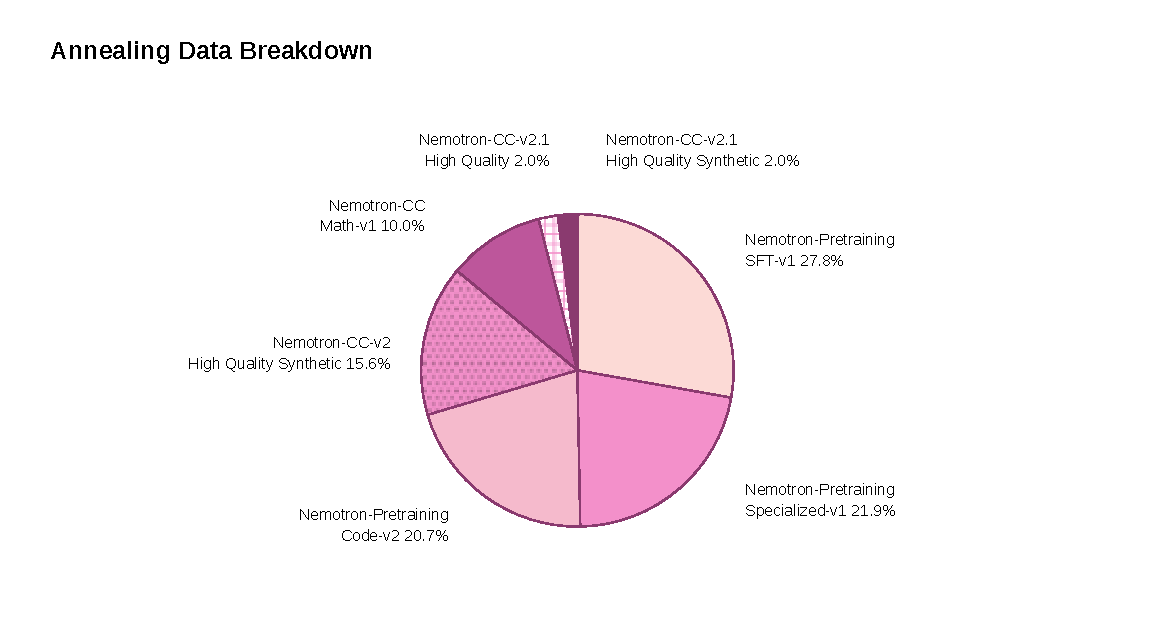
\includegraphics[width=\linewidth]{figures/annealing.pdf}
\caption{Composition of the Stage-2 high-quality annealing data pool: multiple data sources make up the 1.26T-token annealing recipe.}
\label{fig:stage2_data_mix}
\end{figure}
\FloatBarrier

\paragraph{Nemotron-pre-training-SFT-v1.}
We include approximately 351B tokens from Nemotron-pre-training-SFT-v1, a diverse SFT-style dataset of synthetic and curated examples spanning STEM, academic, code, mathematics, and reasoning domains, with multilingual coverage. Its STEM component is expanded from high-quality math and science seeds through iterative generation with Qwen3 and DeepSeek models, producing harder and more varied questions with solutions. The dataset also contains academic question-answer pairs synthesized from undergraduate- and graduate-level texts, as well as MMLU-style general QA and fundamental reasoning data.

\paragraph{Nemotron-pre-training-Specialized-v1.}
We include approximately 277B tokens from Nemotron-pre-training-Specialized-v1, which comprises synthetic data for STEM reasoning, scientific coding, and cross-domain coding, as well as synthetic Wikipedia data and synthetic mathematics textbook data. The STEM reasoning component includes reasoning question-answer demonstrations generated from advanced scientific seed documents, while the scientific coding and cross-domain coding subsets introduce graduate- or research-level programming tasks with structured solutions. This data is intended to strengthen scientific reasoning, mathematical abstraction, and code generation during annealing.

\paragraph{Nemotron-pre-training-Code-v2.}
We randomly sample 60\% of Nemotron-pre-training-Code-v2, yielding approximately 262B tokens. This dataset combines recent GitHub source code, synthetic code-grounded question-answer data, student-teacher dialogues, code-review dialogues, and LLM-rewritten or transpiled source code. The rewriting and transpilation components are designed to improve downstream code generation by increasing stylistic diversity and exposing the model to semantically equivalent code variants.

\paragraph{High-quality synthetic web data.}
We randomly sample 16\% of Nemotron-CC-v2-High-Quality-Synthetic, yielding approximately 197B tokens. This dataset is derived from Nemotron-CC-v2 and contains English web-crawl documents augmented through synthetic rephrasing with Qwen3-30B-A3B. We further include 25B tokens from Nemotron-CC-v2.1-High-Quality-Synthetic, which extends the synthetic high-quality web corpus with newer Common Crawl snapshots and additional rephrased medium- to high-quality documents.

\paragraph{High-quality web data.}
We include approximately 25B tokens from Nemotron-CC-v2.1-High-Quality. This subset incorporates recent Common Crawl snapshots and high-quality data translated into English from multiple languages. Additional LLM-based filtering removes uninformative translated documents. The inclusion of this data preserves exposure to natural web text during the annealing phase.

\paragraph{Mathematics data.}
Finally, we include approximately 126B tokens from Nemotron-CC-Math-v1, using only documents with quality scores of 4 and above. Nemotron-CC-Math-v1 is a high-quality math pre-training corpus built from Common Crawl using a pipeline designed to preserve equations and code, convert mathematical notation to standardized LaTeX, and remove noise. This component is included to strengthen mathematical reasoning and symbolic problem-solving capabilities.
